\section{Exact Oracles in Directed Planar Graphs}\label{exactPlanar}
Previous works have given exact distance oracles for directed planar graphs of size
$O(n^{5/3})$ with query time $O(\lg n)$ \cite{cohen2017fast}. This was improved recently
to use $O(n^{3/2})$ space \cite{gawrychowski2017better}. In the general planar case, we have
bounds that depend on the number of vertices $n$. But in the vertex-labeled case, we can
sometimes win space or obtain better query times by depending on the number of labels
$\ell$. We show one such distance oracle in Section \ref{oracle1}. We also give an oracle
that does not depend on $\ell$, but has better query times in Section \ref{oracle2}.

\subsection{A distance oracle depending on $\ell$}\label{oracle1}
We cannot directly adapt the approach used in \cite{cohen2017fast} and \cite{gawrychowski2017better} to work
for the vertex-labeled case as it requires us to know the target vertex and there might
be many vertices with the same label. We can however use the number of labels $\ell$ to
construct an efficient distance oracle. The idea is store shortest paths for only a subset of the vertices (the boundary vertices of an $r$-division). In the query step, we only need to find the minimal
distance of the shortest paths that pass through the boundary vertices. We give the
following result.
\begin{thm}\label{thm1}
  There is a distance oracle with space $O(n\ell^{2/3)})$, query time $O(\ell^{1/3})$ and
  preprocessing time $\tilde{O}(n\ell^{2/3})$.
\end{thm}
\textbf{The data structure}.
We are given a directed graph $G$, with nonnegative edge lengths and a number of labels
$\ell$. We start by constructing an $r$-division. Remember, we use the $r$-division described in
\cite{klein2013structured}, which guarantees a constant number of holes in each region
and ensures the total number of boundary vertices is $O(n/\sqrt{r})$. Each piece $P$ then
has at most $r$ vertices and $O(\sqrt{r})$
boundary vertices. For each boundary node $b_i$, we store the shortest distance
$\delta(b_i,\lambda)$
for all $\lambda \in L$ in a hash table. For all vertices inside $P$, we store the shortest
distance to all boundary nodes as well as the shortest distance to all labels present in
$P$ in a hash table. \\
\\
\indent \textbf{Query}.
Given the query $Q(v, \lambda)$, if $v$ is a boundary vertex, we can look
up the distance in the hash table for $v$. If $v$ is not a boundary vertex, look up the
distances $\delta(u,v)+\delta(b_i,\lambda)$ for all boundary vertices $b_i$ and the distance
$\delta(v,\lambda)$ stored in the hash table for $v$ and return the minimal distance.

\subsubsection{Analysis}\label{oracle1analysis}
\textbf{Preprocessing}. The $r$-division can be constructed in $O(n)$ time
\cite{klein2013structured}. We need to store distances from all boundary vertices to (potentially)
all other vertices in the graph. Henzinger et al. \cite{henzinger1997faster} gave a $O(n)$
time algorithm for single source shortest path in planar graphs. Using this for all
boundary vertices takes $O(n^2/\sqrt{r})$. We then construct the non-planar graph $G'$, where all
edges between boundary vertices have weight $\delta(u,v)$ for boundary vertices $u$ and
$v$. This information is computed in the previous step and takes $O(n)$ time to
construct as the number of edges we add is $O(r)$ for each of the $O(n/r)$ pieces. To compute distances in the interior of each
piece, we use Fredman and Tarjan's version of Djikstra's algorithm using Fibonacci heaps
\cite{fredman1987fibonacci}. This requires $O(n\lg n + m)$ time for each vertex. Each
piece has $r$ vertices, the number of edges in each piece in the graph $G'$ is also $O(r)$. Using
this implementation for each interior vertex gives us a total running time of $O(n(r\lg r
+ r))=O(nr\lg
r)$. The total preprocessing thus requires $O(n^2/\sqrt{r}+nr\lg r)$ time. \\
\\
\textbf{Space}. For each boundary vertex, we store the distance to all labels. The $r$-division gives us
$O(n/r)$ pieces and ensures we
get $O(\sqrt{r})$ boundary nodes, so this yields
$O(\frac{n}{r}\sqrt{r}\ell)=O(\frac{n}{\sqrt{r}}\ell)$ space. For all other vertices, we
store the distances to all boundary vertices and to all labels within that piece. This
gives us $O(nr)$ space as we can potentially store the distances to all vertices in a
piece $P$. This gives us a total of $O(\frac{n}{\sqrt{r}}\ell+nr)$ space. \\
\\
\textbf{Query}. The query $Q(b,\lambda)$ for a boundary vertex $b$ can be looked up in its hash table in
$O(1)$ time. For the query $Q(v,\lambda)$ for a vertex $v$ not on the boundary, we have
to find the minimal distance $\delta(v,b_i)+\delta(b_i,\lambda)$ for all boundary
vertices in the same piece as $v$, compare it to the distance $\delta(v,\lambda)$ stored in the hash table for $v$
and return the minimal of these two distances. Thus the query time is bounded by the
number of boundary vertices which is $O(\sqrt{r})$. \\
\\
We have a simple trade-off, since we can pick $r$ to be sufficiently small to
achieve constant query time, but this would give $O(n\ell)$ space. However, picking
$r=\ell^{2/3}$ and for $n$ sufficiently large, gives us $\tilde{O}(n\ell^{2/3})$ preprocessing time, $O(n\ell^{2/3})$ space and query time $O(\ell^{1/3})$. This gives us Theorem $\ref{thm1}$.

\subsection{A distance oracle with better query times}\label{oracle2}
We now present a distance oracle which is actually multiple data structures that perform
well depending on $\ell$ and the size of each $\lambda\in L$. We will refer to the
number of a given label by saying the \textit{size} of that label. We can show the following theorem:
\begin{thm}\label{thm2}
  Under the assumption that $G$ does not have $\omega(\sqrt{n})$ labels of polynomial
  size, there is a distance oracle with space $O(n^{3/2})$, query time $O(\text{polylog}(n))$ and
  preprocessing time $\tilde{O}(n^{3/2})$.
\end{thm}
We assume shortest paths are unique, which can be ensured
in linear time \cite{motwani2010randomized}\cite{mulmuley1987matching}. We also assume
the graph is triangulated, which we can do by adding edges with infinite length. \\
Before diving into the data structure, we give the intuition behind the oracle. At high
level, when $k=\text{size}(\lambda)$ for some label $\lambda$ is sufficiently small, we
can perform $k$ queries of the type $Q(u,v)$, where each query takes $O(\lg n)$ time.
When label sizes $k$ are too large (which we know at preprocessing stage), we store the
shortest paths to these labels directly. \\
Computing the shortest paths between two vertices $u$ and $v$ boils down to finding the
hole $h$ that $v$ is contained in and afterwards finding the site (or boundary vertex) that $v$ belongs to in the stored additively weighted Voronoi
diagram $VD^*(u,h)$. It takes $O(\lg n)$ time to locate the hole $h$ and $O(\lg
\sqrt{r})$ to find the site $v$ belongs to. Since we have stored distances to all
vertices for all sites, we can find $\delta(u,v)$ in $O(1)$ time.

\subsubsection{The data structure}
Given the directed planar graph $G$ with non-negative edge length and a number of labels $\ell$ with
$\varepsilon_1 = O(\sqrt{n})$ and $\varepsilon_2=O(\text{polylog}(n))$, we divide our
data structure into the following two cases: \\
\\
\textbf{Case 1:} If $\ell\in [1, \varepsilon_1]$, simply store the matrix of all shortest paths for all nodes to all
labels in the graph. \\
\\
\textbf{Case 2:} If $\ell\in (\varepsilon_1, n]$ and there are $\varepsilon_1$ number of labels that have
polynomial size. \\
First of all, for all labels
$\lambda\in L$, we
store $\text{size}(\lambda)$ in a hash table. We also store, for each label $\lambda_i$,
a hash table that contains all vertices given a label $\lambda_i$. \\
Now define $\mathcal{L}$ as the set of labels
with polynomial size:
\begin{align*}
  \mathcal{L}=\{\lambda\ |\ \text{size}(\lambda)=O(n^\varepsilon)\}
\end{align*}
for $\varepsilon>0$. We store the
shortest paths $\delta(v, \lambda)$ from all vertices $v\in V$ and labels $\lambda\in
\mathcal{L}$ in a hash table. Otherwise, for labels that have size
$\varepsilon_2$, we
use an approach similar to that described in \cite{cohen2017fast} and
\cite{gawrychowski2017better}: \\
\indent The processing stage consists of constructing a $r$-division,
giving us a decomposition tree of $G$. For all pieces $P=(V_P, E_P)$ at some
step in the decomposition, we store shortest path trees for all boundary vertices of $P$.
Additionally, we store distances $\delta(u,b_i)$ in the entire graph $G$ for all $u\in V$ and boundary vertices $b_i$. Now
consider the step where $P$ is split into two smaller pieces $Q$ and $R$. For each
vertex, we record if it belongs to $Q$ or $R$ or the separator $C$. Recall the definition of an
additively weighted Voronoi diagram from Section \ref{techniques}. For all vertices $u\in
Q$ and hole $h$ of $R$, we store an additively weighted
Voronoi diagram $VD^*(u,h)$. We will explain the details of the diagram when we explain
the query in Section \ref{oracle2query}. We store the
same information with $Q$ and $R$ interchanged. \\
In order to explain how the
query works, for each vertex $v*$ of $VD^*$, we add three artificial edges with zero
weight to the three vertices adjacent
to the face in the primal graph that correspond to $v^*$. Note that the three vertices all
belong to different Voronoi cells and that we have stored the shortest paths from the site they
belong to. Figure \ref{vd2} illustrates the
situation for a single hole $h$ and vertex $v^*$ in $R$.

\begin{figure}[h!]
  \centering
  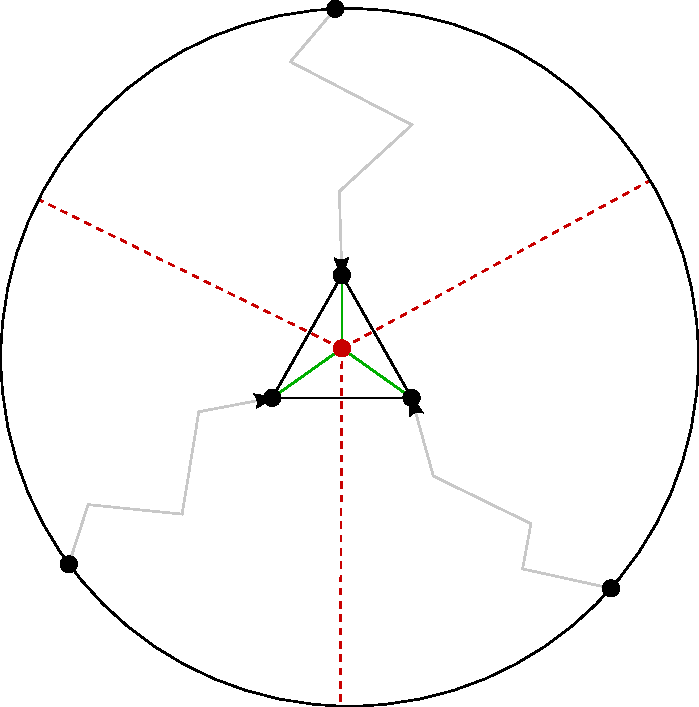
\includegraphics[width=0.66\textwidth]{figs/vd2.pdf}
  \caption{Illustration of $VD^*$ and a vertex in the graph. The vertex $v^*$ is given in
  red and vertices of $G$ are given in black. The edges of $VD^*$ are given by red dashed
  lines and the edges
of $G$ are black. The artificial edges with zero weight we add are given in green. The
shortest path from the sites of the adjacent Voronoi cells to the vertex adjacent to the
face corresponding to $v^*$ is given in grey.}
    \label{vd2}
\end{figure}

\subsubsection{Query}\label{oracle2query}
Depending on the case that $G$ falls under, we do the following for the
query $Q(v, \lambda)$: \\
\\
\textbf{Case 1:} Look up the distance in the hash table stored for $v$. \\
\\
\textbf{Case 2:} The query is $Q(u,\lambda)$. If the size of $\lambda$ is polynomial,
we can look up the distance stored the hash table for that label in $O(1)$ time.
Otherwise the size of $\lambda$ is $\varepsilon_2$ and we refer to the data structure
described above. Let $\mathcal{V}\subset V$ be the set of vertices with label $\lambda$.
For each $v\in \mathcal{V}$, we perform the query $Q(u,v)$:\\
When a region $P$ is split into two regions $Q$ and $R$ with a separator $C$, if
either $u$ or $v$ belongs to $C$, then we can look up the distance in $O(1)$ time since
we have stored all distances to and from boundary vertices. If both belong to the same
smaller piece, we go into that piece. The last case is when $u\in P$ and $v\in Q$. In this
case, we can locate the hole $h$ which contains $v$. Since we have stored the
additively weighted Voronoi diagram $VD^*(u,h)$, we perform a point location query to
determine the site which $v$ belongs to in $VD^*$. An important property of $VD^*$ is that Lemma
\ref{lemma2} holds.
\begin{lemma}\label{lemma2}
  $VD^*$ is a tree.
\end{lemma}
A proof is found in Appendix \ref{a2} by Gawrychowski et al.
\cite{gawrychowski2017better}.  \\
The idea is then to construct a centroid decomposition of $VD^*$. To locate the
Voronoi cell $v$ belongs to, it is sufficient to locate a terminal edge $e^*$ of $VD^*$, so that
$v$ is in one of the two Voronoi cells adjacent to it. Now consider a vertex $v^*$
adjacent to three cells. Let $y_j$ be the three vertices in the primal graph adjacent to
the face of $v^*$. We can determine in $O(1)$ time which site is closest to $v^*$ and if it is
left or right of the shortest path, $p_i$, from site $s_i$ to $v^*$ (using preorder
numbers and a LCA data structure \cite{bender2000lca}). Say $s$ is the site closest to
$v^*$, the boundary of the cell contains two edges of
$VD^*$ that we can traverse from $v^*$. Depending on the position of $v$ relative (left or right) to the shortest path,
we traverse one of the edges. If $v$ is directly on the shortest path, we can
deduct it belongs to the Voronoi cell of $s$ (refer to Figure \ref{vd1}). Namely, Lemma
\ref{lemma1} holds:
\begin{lemma}\label{lemma1}
  Let $s$ be the site such that $v\in \text{Vor}(s)$. If $T^*$ contains all edges of
  $VD^*$ incident to $\text{Vor}(s)$, and if $v$ is closer to site $s_i$ than to the
  sites $s_{i-1}$ and $s_{i+1}$ (indices modulo $3$), then one of the following is true:
  \begin{itemize}
    \item $s=s_i$
    \item $v$ is right of $p_i$ and all boundary edges of $\text{Vor}(s)$ are contained
      in in $T_i^*$
    \item $v$ is left of $p_i$ and all boundary edges of $\text{Vor}(s)$ are contained
      in in $T_{i+1}^*$
  \end{itemize}
\end{lemma}
\noindent A proof of Lemma \ref{lemma1} by Gawrychowski et al. \cite{gawrychowski2017better} is
found in Appendix \ref{a1}. \\
We continue this approach until we find a
terminal edge $e^*$, from which we can tell which cell $v$ belongs to by comparing the
distances to both sites.

\begin{figure}[h!]
  \centering
  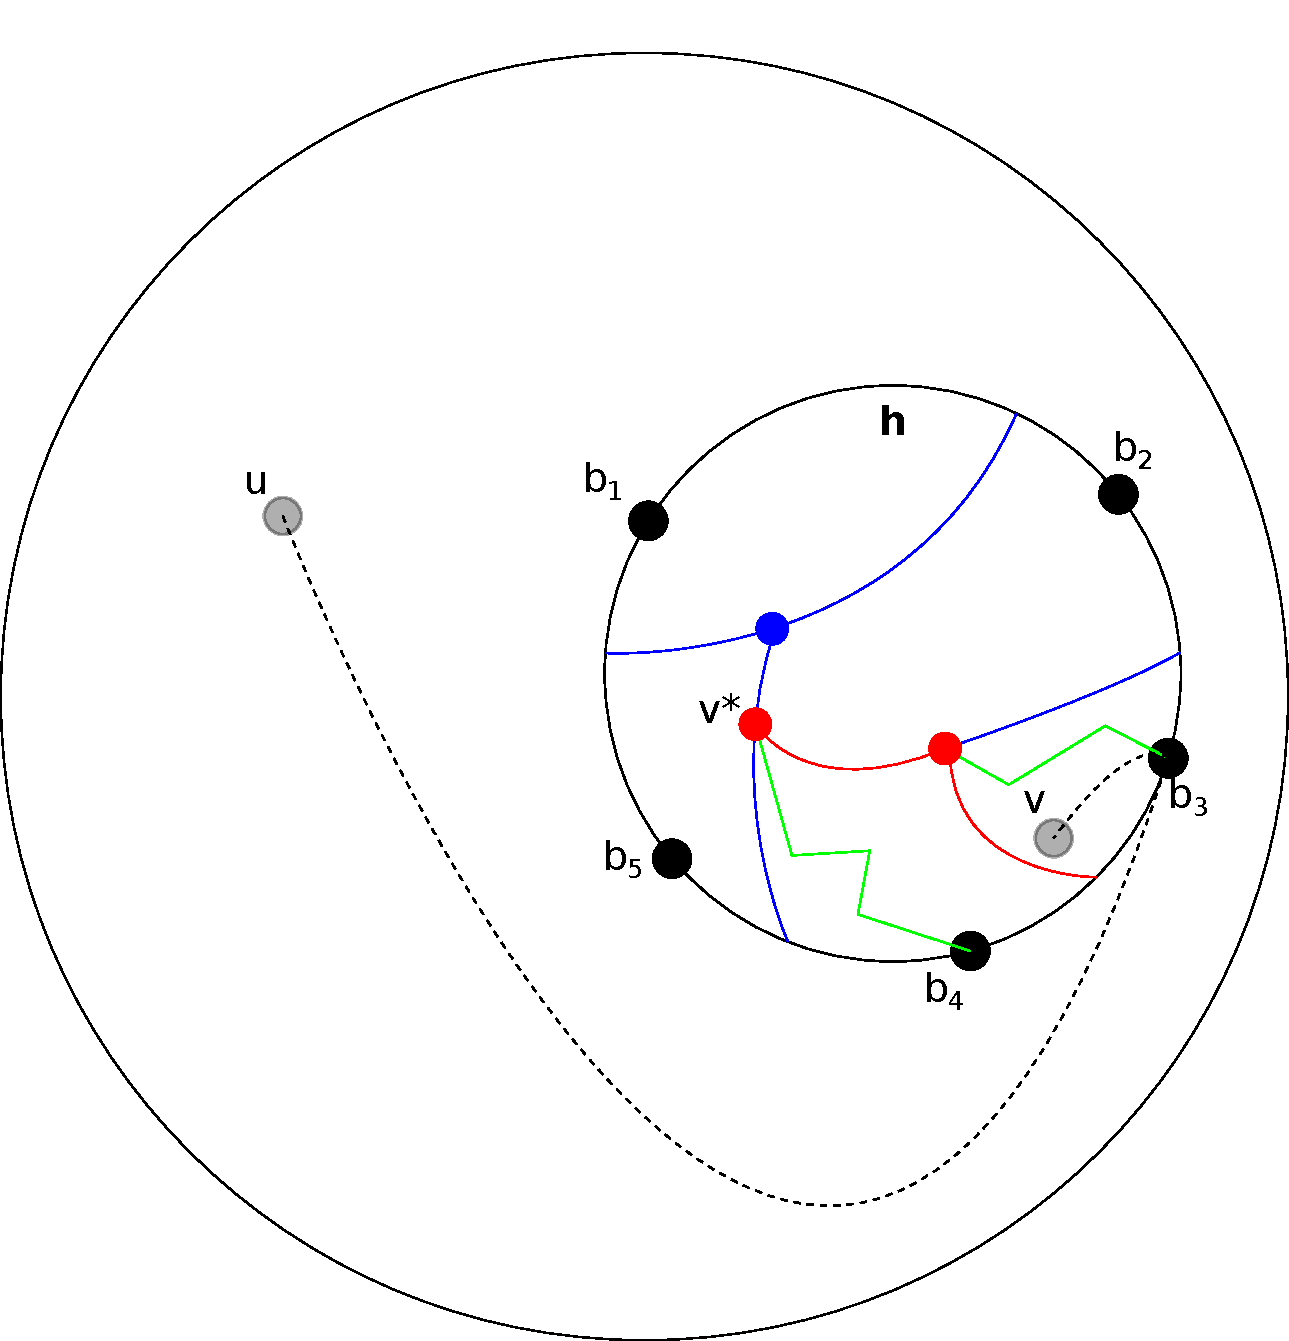
\includegraphics[width=0.66\textwidth]{figs/vd1.pdf}
  \caption{Illustration of how a query $Q(u,v)$ works. First, we determine which hole $h$
    that $v$
  belongs to. We then traverse our centroid decomposition of the
  additively weighted Voronoi diagram $VD^*(u,h)$ (in blue) starting at the vertex $v^*$ given in
red. We compare the distances from $u$ to $v$ through the three sites ($b_2$, $b_4$,
$b_5$). Say the shortest distance is through $b_4$, we need to locate $v$ relatively to
the shortest path from $b_4$ to $v^*$ (in green). Since $v$ is
located right of this path, we traverse the edge given in red. Again, we compare the
distances from $u$ to $v$ through the three sites $b_2$, $b_3$ and $b_4$. The shortest
path goes through $b_3$ and $v$ is located left of the shortest path from $b_3$ to the
Voronoi vertex, so again we traverse the corresponding edge. Since this is a terminal
edge, we can determine that $v$ belongs to the Voronoi cell of $b_3$.}
    \label{vd1}
\end{figure}

\subsubsection{Analysis}\label{oracle2analysis}
\textbf{Preprocessing}. \\
\textit{Case 1}. We need to store shortest paths from all vertices to the nearest
$\lambda$-labeled vertex for all labels. To achieve this, we construct the graph $G'$, where the
direction of all edges are reversed in $O(n)$ time. For each label $\lambda_i$, we add a
super vertex and connect all vertices with label $\lambda_i$ to it with weight zero. Call this non-planar
graph for $G'(\lambda_i)$. We then perform Djikstra
\cite{fredman1987fibonacci} to compute SSSP from the super vertex in $G'(\lambda_i)$ in
$O(n\lg n)$ time. The distances to each vertex correspond to the shortest path
$\delta(u,\lambda_i)$ for all vertices $u$. We perform this step $\ell$
times, so the total preprocessing time is $O(n\ell \lg n)$. Since $\ell=O(\sqrt{n})$, this
yields $\tilde{O}(n^{3/2})$ preprocessing time. \\
\\
\textit{Case 2}. First consider the case where labels have polynomial size. For all
vertices, we need to store the shortest path to these labels. By the same analysis of case 1,
we get that it takes $\tilde{O}(n^{3/2})$ time to compute these distances as we expect at
most $O(\sqrt{n})$ labels with polynomial size. \\
The $r$-division along with its decomposition tree is constructed in $O(n)$
time \cite{klein2013structured}. Consider a step where the graph is separated into $Q$
and $R$. To compute all additively weighted Voronoi diagrams for every node $u\in
Q$, hole $h$ of $R$, we need all
shortest path to and from boundary vertices of $h$. Lemma \ref{rdivlemma} tells us that there are
$O(\sqrt{n})$ boundary vertices at any level in the decomposition, so computing the shortest path trees for all
boundary vertices can be done in $O(n^{3/2})$ time. To compute all shortest path \textit{to} boundary vertices, we construct the graph
$G'$, which is the graph obtained by changing the direction of all edges of $G$. Since
$G$ is planar, it has $O(n)$ edges, so this can be achieved in $O(n)$ time. We then
compute all shortest path trees rooted at boundary vertices in $O(n^{3/2})$ time. The
distances $\delta(b,u)$ in $G'$ for a boundary vertex $b$ and interior vertex $u$ are then equal
to the distance $\delta(u,b)$ in $G$. We get the same result with $Q$ and $R$
interchanged. This takes a total of $O(n^{3/2})$ time. The diagrams are constructed in
$O(r)$ time and extended in $O(\sqrt{r})$ time to support point location
\cite{gawrychowski2017better}. We also create a hash table of size $O(n)$ in $O(n)$ time that can return all vertices with a given label \cite{fredman1984storing}.
Likewise, the hash table keeping track of the size of labels takes $O(n)$ time to
create and takes $O(\ell)$ space. Thus, the total time for preprocessing is $\tilde{O}(n^{3/2})$. \\
\\
\textbf{Space}. \\
\textit{Case 1}. We store $\ell$ distances for each vertex $v$. Since $\ell=O(\sqrt{n})$, this
yields space $O(n^{3/2})$. \\
\\
\textit{Case 2}. Since we assumed that there are no more that
$O(\sqrt{n})$ labels of size $\omega(\text{polylog}(n))$, the hash table storing the
distances to these labels cannot require more than $O(n^{3/2})$ space. The hash table
storing the size of all labels require $O(\ell)$ space. The hash table storing all
vertices, given their label, requires $O(n)$ space. Additionally, every time we
separate the graph into $Q$ and $R$, we need to record whether vertices belong to $Q$ or
$R$ or the separator $C$. Since the recursive decomposition has depth $O(\lg n)$, the
space required for this is $O(n\lg n)$. \\
We also need to store all distances $\delta(b,v)$ and $\delta(v,b)$ for all
boundary vertices $b$. Since the number of boundary vertices is $O(\sqrt{n})$, this
requires a total of $O(n^{3/2})$ space. \\
Lastly, we need to store additively weighted Voronoi diagrams for a vertex $u\in Q$ and
hole $h$ of $R$. Recall that we can store an additively weighted Voronoi diagrams in
$O(\sqrt{r})$ space. Since we store $O(1)$ diagrams (because each piece has $O(1)$ holes) for
all vertices in the entire graph $G$, this requires a total space of $O(n\sqrt{r})$. The
same is true with $Q$ and $R$ interchanged. \\
Thus the total space required is $O(n^{3/2}+\ell+n\lg n+n\sqrt{r})=O(n^{3/2})$. \\
\\
\textbf{Query}. \\
\textit{Case 1}. We look up the distance in the hash table in $O(1)$ time.\\
\\
\textit{Case 2}. All labels have size $O(\text{polylog}(n))$. The point location method
described
above takes $O(\lg n)$ time as we descend into pieces in the recursive decomposition with depth
$O(\lg n)$. Since the trees constructed for each additively weighted Voronoi diagram has
depth $O(\lg \sqrt{r})$ and $r<n$, this term does not add to the query time. However,
there can be up to $O(\text{polylog}(n))$ vertices of a given label, which means we have
to do $O(\text{polylog}(n))$ different point locations and take the minimal distance
found. This
yields a total query time of $O(\text{polylog}(n))$. \\
\\
The data structure and analysis of case 1 gives combined with the data structure and
analysis of case 2 gives us the distance oracle from Theorem \ref{thm2}.

\subsubsection{Removing the assumption on the distribution of the labels}
Unfortunately, handling the case when the graph can have $\omega(\sqrt{n})$ labels with
polynomial size proved difficult. However, to complete the distance oracle for all
distributions of $L$, we can loosen up on either space or query time. \\
\\
If we allow more space, we can store the distance to polynomial sized labels directly. In
worst case, this would be the same as the trivial case, requiring $O(n\ell)$ space. \\
\\
If we allow worse query time, first note that we cannot have more than $O(\sqrt{n})$
labels of size $\omega(\sqrt{n})$. So for all labels with size $\omega(\sqrt{n})$, we can
handle as in case 1. However, for all other labels, $\lambda$, with polynomial size $o(\sqrt{n})$, by the same
approach as in case 2, we would need to make point to point distance queries for all the
vertices with label $\lambda$ . This requires $\tilde{O}(\text{size}(\lambda))$, which in
the worst case is $\tilde{o}(\sqrt{n})$.

\subsubsection{The trade-off}\label{exactoracletrade}
The two described data structures have different advantages. When the desired space
allocation $S$ is in the range $[n,n^{3/2})$ or if $\ell=o(\sqrt{n})$, we use the first
  data structure. The trade-off we achieve in that was $O(nr\lg r)$ for preprocessing,
  $O(n\ell/\sqrt{r})$ for space and $O(\sqrt{r})$ for query time. In
  the extreme cases, we have $O(n\ell)$ space or $O(\sqrt{n})$ query time.  \\
Note that the space-query product is no better than the trivial $n\ell$ solution where we
store shortest paths from all vertices to all labels in a matrix and have $O(1)$ queries. \\
The trade-off for the second oracle with the
assumption on labels is, given a desired space allocation $S$ when $S\geq n^{3/2}$, we get a
query time of $O(\text{polylog}(n))$ with preprocessing $\tilde{O}(n^{3/2})$. In this
case, the space-query product does beat that of the trivial solution whenever
$\ell=\omega(\sqrt{n})$. In case $\ell=O(\sqrt{n})$, the data structure does the same as
in the trivial solution.
